\chapter{Fundamentos Teóricos e Conceptos Previos}

O desenvolvemento dunha aplicación web non é algo trivial e máis se temos en conta todas
as peculiaridades que este proxecto contén. Para a súa comprensión é preciso coñecer unha
serie de conceptos teóricos que se expoñen a continuación:

\section{Arquitectura web}
	No proxecto séguese unha Arquitectura Web baseada no modelo cliente-servidor, que 
	consiste nun lado servidor que distribúe os recursos como poden ser o contido multimedia
	(vídeos, imaxes, etc) ou as páxinas web ao outro lado, o cliente, que tipicamente corre 
	nun navegador web interpretando as páxinas html e o código javascript asociado a estas.
	
	Neste caso a parte servidor estará dividida en dúas compoñentes claramente diferenciadas,
	o sistema para a análise do comportamento e a aplicación web que permitirá o acceso a este, 
	os fundamentos de ámbalas dúas partes pódense ver no diagrama 
	\ref{fig:ArqSistemaSimplificado} e os fundamentos nos que están baseadas explícanse a 
	continuación.
	
    \begin{figure}[htp]
    \begin{center}
        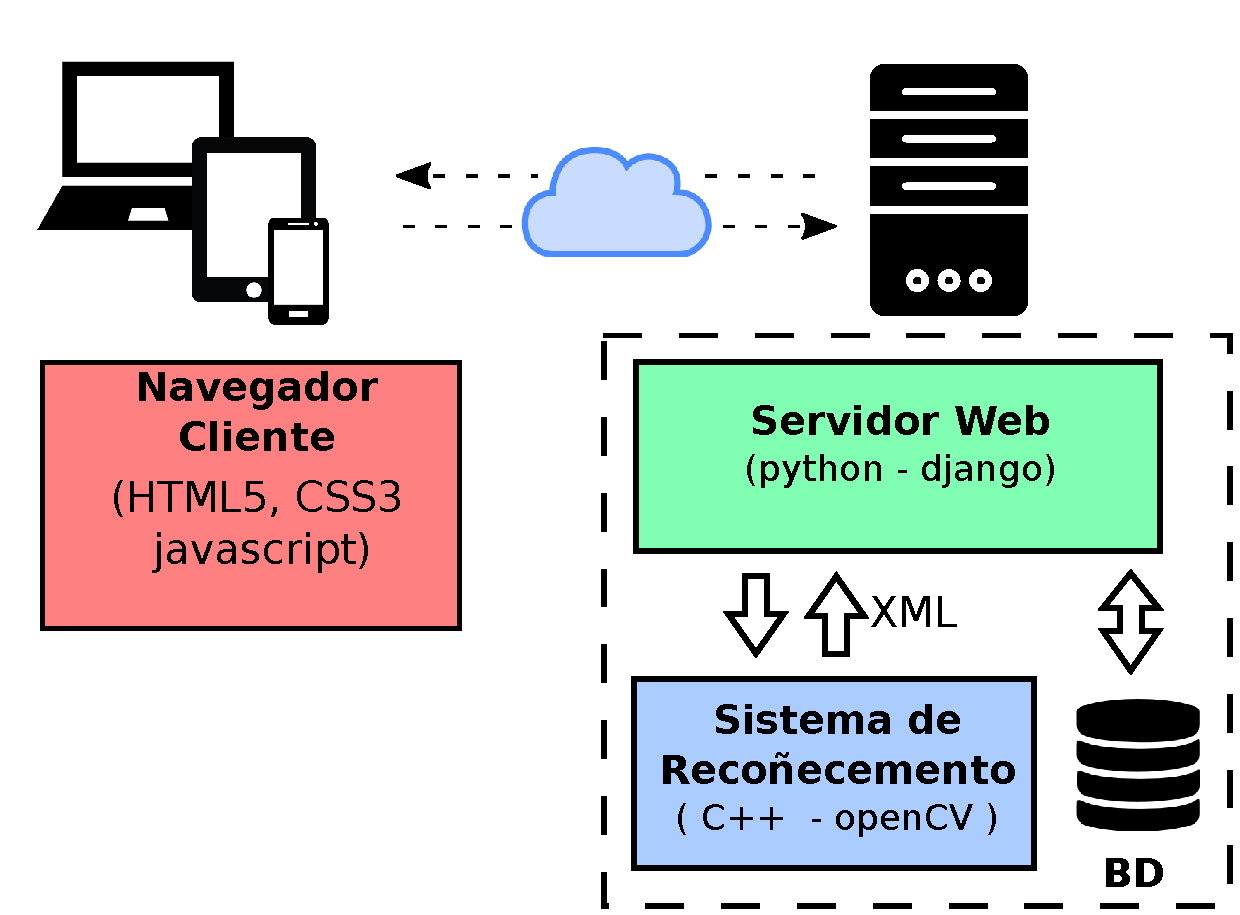
\includegraphics[scale=0.45]{figures/ArqSistemaSimplificado.pdf}
        \caption{Diagrama simplificado da Arquitectura do Sistema}
    \label{fig:ArqSistemaSimplificado}
    \end{center}
    \end{figure}
	
\section{Análise do comportamento}
	É un dos campos de investigación mas activos hoxe en día. A idea principal na que se 
	centran estes sistemas como o que nos ocupa é a de detectar calquera acción levada a 
	cabo polos obxectos involucrados nunha escena de vídeo. Un obxecto é calquera cousa 
	que debe ser seguida, polo que dependendo do tipo de problema estes obxectos poden 
	ser dunha natureza ou doutra.
	O tipo de accións a detectar tamén depende da tipoloxía do sistema, xa poden ser
	comportamentos individuais( camiñar, correr, loitar...) ou grupais (reunirse, abandonar
	un grupo de persoas...).
	
	Tanto neste proxecto como nos sistemas para a análise do comportamento en xeral, 
	pódense discernir tres tarefas importantes que colaboran entre si \cite{brais-thesis}:
	
	\begin{itemize}
	
		\item{\textbf{Detección de Obxectos:}}\label{cap:DeteccionObxetos} Partindo dunha secuencia de vídeo como 
		entrada obtéñense os distintos obxectos que aparecen en cada fotograma da escena.
		Para este fin empréganse técnicas de visión por computador.
		
		%Aqui podríame extender falando da Substracción de Fondo, o Fluxo Óptico e os Sistemas de alto Nivel
		
		\item{\textbf{Seguimento de Obxectos:}} A partires da información obtida na detección, asígnanselle 
		identificadores a cada obxecto detectado no vídeo, agrupando se procede distintos
		obxectos baixo o mesmo identificador en caso de considerarse que estes obxectos forman
		parte de un grupo ou unha mesma detección.
		
		% Aquí podría falar das aproximacións por apariencia, filtro de Kalman, filtro de Partículas ..
		
		\item{\textbf{Análise do comportamento de Alto Nivel:}} Unha vez obtida a información dos 
		dous pasos anteriores pódese catalogar o comportamento de cada detección empregando
		técnicas de recoñecemento de patróns.
	
	\end{itemize}	
	
	Os resultados máis destacables destas técnicas cos que a aplicación terá que traballar serán:
	\begin{itemize}
		\item A lista de obxectos detectados para cada un dos fotogramas e a súa posición neles
		\item A traxectoria de cada un dos obxectos detectados
		\item O grao de anormalidade da traxectoria seguida por un obxecto en cada un dos fotogramas
	\end{itemize}
	
	Estas tres tarefas agrupanse baixo un mesmo sistema ao que chamaremos Sistema de Recoñecemento
	e que xunto co servidor web, apoiado nos fundamentos que veremos a continuación, forman o lado
	servidor deste proxecto. 
	
\section{Programación Web}

	A programación web de aplicacións de carácter empresarial require do coñecemento da rede, ademais
	do de unha serie de ferramentas e estratexias para chegar a un deseño sostible e de calidade.
	
	A arquitectura clásica das aplicacións web pódese ver no gráfico \ref{fig:ArquitecturaAppWeb}, 
	ela contén unha parte cliente que se executa no navegador do usuario, e unha parte servidor que
	á súa vez acostuma a dividirse nunha BD (Base de Datos) que almacena a información precisa, unha 
	capa modelo que reflexa o modelo de negocio da nosa aplicación tipicamente nalgunha linguaxe 
	de programación e por último unha capa de IU Web (Interface de Usuario Web) que se encarga de 
	transformar os datos da capa modelo a un formato web comprensible polo cliente e viceversa.
	
	\begin{figure}[htp]
	\begin{center}
		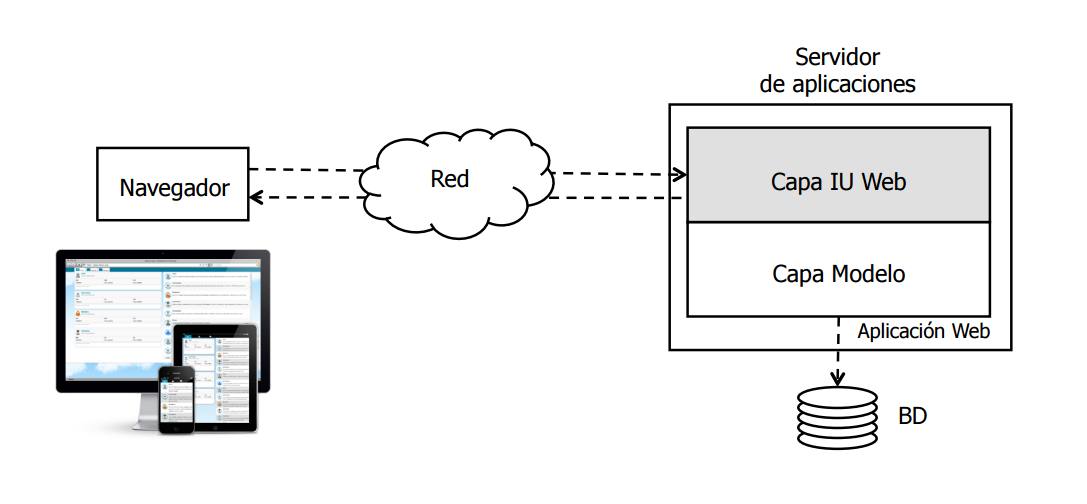
\includegraphics[scale=0.35]{figures/ArquitecturaAppWeb.png}
		\caption{Clásica arquitectura dunha aplicación web empresarial}
	\label{fig:ArquitecturaAppWeb}
	\end{center}
	\end{figure}

	As técnicas e estratexias máis importantes á hora de construír unha aplicación web relátanse nos
	puntos subseguistes:
	
	\subsection {Desenvolvemento Áxil}
		Para reducir custos e poder proporcionar solucións rápidas é preciso que as 
		aplicacións web's de carácter empresarial se leven a cabo en pouco tempo e con
		bos principios de enxeñaría, a isto contribúen en gran medida as estratexias de programación 
		que se explican a continuación e que se ven no diagrama \ref{fig:fundamentos}.
		
    \begin{figure}[htp]
    \begin{center}
        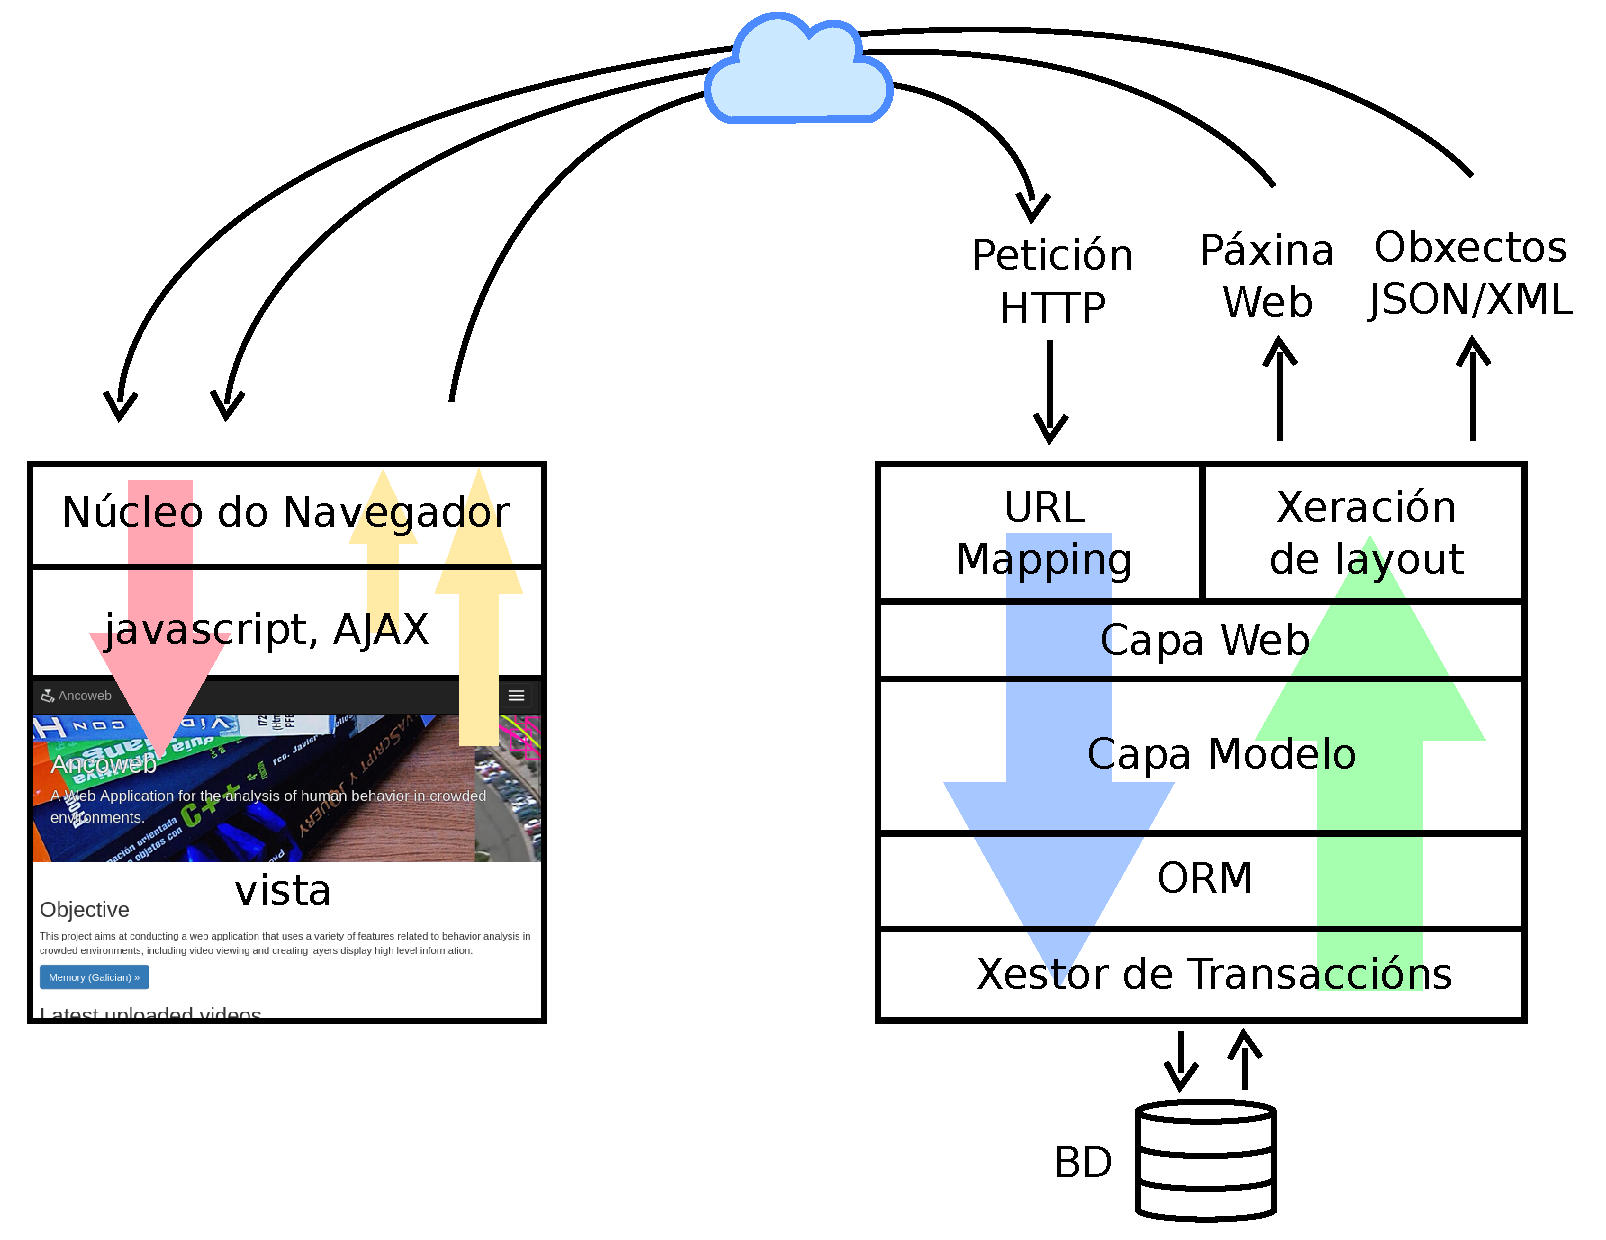
\includegraphics[scale=0.4]{figures/fundamentos.pdf}
        \caption{Diagrama sobre os conceptos de programación}
    \label{fig:fundamentos}
    \end{center}
    \end{figure}
		
        \subsubsection{Soporte para transaccións}
            Unha transacción nun Sistema Xestor de Base de Datos (SGBD) é un conxunto de ordes que
            se executan formando unha unidade de traballo, de forma invisible e atómica. 
            As transaccións cobran gran importancia nas aplicacións web debido á inestabilidade 
            da rede e á concorrencia dos distintos clientes conectados, polo que é axuda a un 
            desenvolvemento moi áxil que a tecnoloxía traia a súa xestión integrada.
        
        \subsubsection{Object-Relational Mapping (ORM)}
            Os mapeado obxecto-relación é unha das técnicas de programación que máis velocidade imprimen
            na construcción de webs, xa que converte os datos dunha linguaxe Orientada a Obxectos (OO) a 
            datos de un sistema relacional no que son persistidos e viceversa, aforrando ao programador
            o traballo de ter que programar o código para esta tarefa. É desexable pois que a tecnoloxía
            a empregar dispoña dun mapeador obxecto-relacional ben integrado, algúns exemplos disto poden
            ser: a combinación Java+Maven+Hibernate, o EF(Entity Framework) de Microsoft ou os Models de Django.
        
        \subsubsection{Xestión de Layout}
            Tamén resulta moi practico dispoñer dunha linguaxe de plantilla que permitan xerar contido
            html ben estruturado dinamicamente. Algúns exemplos son o Sistema de Templates de Django, o 
            Sistema JSP de Spring, a libraría Thymeleaf ou os compoñentes de ASP.NET. Todos eles axudan 
            a xerar contido HTML de xeito sinxelo e escalable que logo será enviado ao cliente. De
            tódolos xeitos esta parte cliente as veces precisa comunicarse co servidor sen que sexa 
            preciso unha recarga da páxina e para elo empregase AJAX.
		
    \subsection{AJAX}
		AJAX ou Asynchronous JavaScript And XML é unha tecnoloxía da web empregada para crear 
		aplicacións interactivas, estas aplicacións executanse no navegador dos usuarios mentres 
		manteñen unha comunicación asíncrona co lado servidor en segundo plano. Normalmente 
		empregase javascript coma linguaxe para a realización das chamadas asíncronas en combinación
		con algunha linguaxe para a definición de obxectos como XML ou JSON, para as que ademais os
		propios navegadores adoitan a facilitar ferramentas de parsing.
		
	\subsection{Outras cuestións da web}
		A maiores existe toda unha gama de outras funcionalidades que cobran importancia cando deseñamos
		e construímos unha web como o manexo de erros nos formularios, internacionalización (i18n), 
		visualización de grande cantidades de datos (en listas ou táboas), seguridade...
		
		
\section{O Vídeo}
    O vídeo permite gravar, procesar, almacenar e transmitir información en forma de 
    imaxe en movemento, esta imaxe en movemento soe estar composta por unha serie de imaxes 
    estáticas chamadas fotogramas, que se manexan a unha velocidade alta causando o efecto de que o
    que se está a ver está en movemento.
    
    Non obstante o vídeo en formato electrónico non almacena necesariamente todas as imaxes de forma
    individual xa que isto suporía moita información redundante. En lugar disto empréganse técnicas
    de codificación-decodificación (codec's) que comprimen e descomprimen os datos para facilitar o
    seu manexo.

    \subsection{Codec's}
        Os codec's teñen como función principal a de transformar unha sinal de vídeo para que poida
        ser visto. A maioría dos codec's provocan con cada transformación unha perda de información
        para conseguir un tamaño final o máis pequeno posible, estes codec's chámanse lossless (con 
        perdida) e a pesares de que perden calidade soe compensar pola cantidade de espazo que 
        aforran ao comprimilo vídeo.
        
        A parte de este fenómeno da compresión tamén cobra moita importancia outros aspectos 
        relacionados co vídeo como a reprodución e sincronización de son, os subtítulos do vídeo,
        as imaxes representativas deste... Todo isto depende do formato no que se almacene o vídeo.
        
    \subsection{Formato de Vídeo}
        O formato dun vídeo determina como se almacenan os distintos tipos de información involucrada
        como as imaxes que poden estar codificadas en varios codec, o son, os subtitulos...
        este formato correspondese cunha extensión específica do arquivo que o contén, como por 
        exemplo:
        
        \begin{itemize}
        \item \textbf{AVI (Audio Video Interleaved):} 
            Sendo un dos formatos máis famosos pode conter un vídeo dunha calidade excelente pero
            soe requerir dunha gran capacidade. Os codec's que se soen empregar neste formato pola 
            súa capacidade de compresión e calidade aceptable son DivX e XviD, inda que tamén se 
            permiten outros como DV(Digital Video), CinePak... 
            
        \item \textbf{MKV (Matroska):}
            É un formato de código aberto que basea o seu nome nas clásicas bonecas Matrioskas. Ten
            capacidade para conter tanto vídeo, son e subtitulos en diferentes idiomas, empregandose
            como códec de video normalmente algunha implementación de H.264, como por exemplo x264. 
            Mentres que para o son é habitual empregar o codec de audio Vorbis.

        \item \textbf{ WebM (Google, 2010):}
            Un dos formatos máis recentes é o WebM (WebMovie), un proxecto lixeiramente baseado en 
            Matroska adquirido e liberalizado por Google en 2010 co obxectivo de empregalo con HTML5
            como estándar libre. O formato ten un excelente rendemento e xunto ao codec VP9, motivo
            polo cal forma parte dos recomendados pola W3C.
            
        \item \textbf{Formato OGG (Xiph.Org, 1993):} 
            O formato contedor OGG é un formato libre deseñado para incluír vídeo, son, 
            subtítulos e metadatos. O vídeo en este formato soe estar codificado co codec Theora, 
            que se basea nunha versión liberada de VP3. Tamén se emprega para este tipo de 
            empaquetado a extensión .OGV, mais o que marca o estandar é a extensión .OGG.  
            
        \item \textbf{MP4 - MPEG (Moving Pictures Expert Group):}
        
        O  Moving Picture Experts Group (MPEG) é un grupo de expertos da ISO (Organización 
        Internacional de Normalización) e da Comisión Electrotécnica Internacional (IEC) para
        crear estándares en canto ao mundo do audio e o vídeo.
        
        Froito do traballo deste grupo naceron os formatos MPEG-1 (calidade CD), MPEG-2 (calidade 
        DVD), MPEG-3 (orientado ao audio MP3) e MPEG-4 que é o que máis nos interesa xa que vai 
        enfocado á compresión de vídeo e son na web, podendo incluír tamén subtítulos ou imaxes de 
        referencia. O ficheiros de este último formato teñen extensión .mp4.

        \end{itemize}


    \subsection{Streaming de Vídeo}
        Dado que este proxecto está centrado no tratamento de vídeo, é de especial importancia ver 
        de que xeitos podemos distribuílo e reproducilo a través da rede. A estes efectos existen dúas
        grandes alternativas que varían en canto ao seu grao de escalabilidade, dificultade de 
        implementación, e calidade final do servizo:
        
        \subsubsection{Pseudo Streaming ou Descarga Progresiva}
            Consiste na descarga do vídeo por fragmentos, típicamente empregando o protocolo HTTP. 
            Neste formato, o reprodutor vai acumulando fragmentos de vídeo ata obter os precisos como 
            para comezar a reprodución, mais se o ancho de banda fose insuficiente, o vídeo remataría
            por pararse. Este sistema é o empregado por servizos como YouTube, Vimeo, DailyMotion...
            
            Será a opción empregada por motivos de simplicidade, mais compre explicar tamén o verdadeiro 
            Streaming, xa que é a diferenza do pseudo-streaming pode ser empregado para a emisión de
            contido en directo como o dunha cámara de seguridade.
            
        \subsubsection{Streaming}
        \label{sec:streaming}
            O verdadeiro streaming ( do inglés True Streaming) consiste na emisión en directo do 
            contido multimedia a través da rede, que o reprodutor reproduce no momento que recibe.
            Este outro xeito de distribuír vídeo, apoiase en axustar a calidade do vídeo ao ancho de
            banda do que dispón o cliente, evitando así interrupcións na reprodución.
            
            O protocolo máis destacable á hora de empregar este tipo de streaming é RTSP (Real-Time
            Streaming Protocol) que operando a nivel de aplicación permite controlar un ou varios fluxos 
            sincronizados de contido multimedia como se pode ver na figura \ref{fig:RTPS-diagram}.
            
            Por unha parte RTSP soe empregar o Real-Time Transport Protocol (RTP) sobre UDP(User 
            Datagram Protocol) para o transporte de contido multimedia, maximizando así o emprego 
            da rede pero sen garantir un mínimo na calidade do servizo.
            
            E por outra parte RTSP emprega o Real-time Control Protocol (RTCP) sobre TCP(Transmission 
            Control Protocol) para a transmisión periódica de paquetes de control da sesión, o
            diagnóstico de fallos e o control de la calidade da transmisión.
            
            \begin{figure}[htp]
            \begin{center}
                
\includegraphics[scale=0.6]{figures/RTPS-diagram.png}
                \caption{Diagrama conexión RTPS}
            \label{fig:RTPS-diagram}
            \end{center}
            \end{figure}
            
            RTSP asemellase a HTTP no formato das peticións/repostas e na sintaxe, pero dispoñendo 
            dun estado que permite tanto a clientes como a servidores facer peticións.

            Tamén existen outros protocolos propietarios como MMS (Microsoft Media Server)ou RTMP 
            (Real-Time Messaging Protocol) e RTMFP (Real-Time Media Flow Protocol) de Adobe.
            